\documentclass[12pt,a4paper]{article}

\usepackage[utf8]{inputenc}
\usepackage[T1]{fontenc}
\usepackage[english]{babel}
\usepackage[margin=2.5cm]{geometry}
\usepackage{graphicx}
\usepackage{fancyhdr}
\usepackage{hyperref}
\usepackage{enumitem}
\usepackage{lastpage}
\usepackage{titlesec}
\usepackage{setspace}

\hypersetup{
  colorlinks=true,
  linkcolor=black,
  urlcolor=blue,
  citecolor=black,
  pdfauthor={Pedro Castro},
  pdftitle={Bomberman}
}

\graphicspath{{images/}}

\pagestyle{fancy}
\fancyhf{}
\rfoot{\small \thepage\ /\ \pageref{LastPage}}
\renewcommand{\headrulewidth}{0pt}

\titlespacing*{\section}{0pt}{1.5\baselineskip}{0.5\baselineskip}
\titlespacing*{\subsection}{0pt}{1\baselineskip}{0.25\baselineskip}

\onehalfspacing%

\newcommand{\coverpage}[4]{
  \begin{titlepage}
    \centering
    \vspace*{1.5cm}

    {\bfseries\Large Faculty of Engineering — University of Porto}\\[1.5cm]

    
\includegraphics[width=0.5\textwidth]{feup.png}\\[1.5cm]

    {\Huge \bfseries #1}\\[1cm]

    \if\relax\detokenize{#2}\relax\else
      {\Large #2}\\[1cm]
    \fi

    \vspace*{\fill}
    \if\relax\detokenize{#3}\relax\else
      \includegraphics[width=0.5\textwidth]{#3}
    \fi
    \vspace*{\fill}

    {\large\bfseries\begin{tabular}{c} #4 \end{tabular}}\\[1cm]

    {\large \today}

    \vspace*{1cm}
  \end{titlepage}
}

\begin{document}

\coverpage%
  {Bomberman}
  {A Bomberman clone built in C for MINIX-LCOM.}
  {logo.png}
  {Nuno Gomes\\Pedro Castro\\Vasco Lemos}

\clearpage
\tableofcontents
\clearpage

\section{Project Goal and Description}
The primary goal of this project was to design and implement a functional replica of the classic game \textit{Bomberman}, specifically tailored for the MINIX operating system and written in C. This project was developed as part of the LCOM course at the Faculty of Engineering of the University of Porto. Players must navigate through maze-like levels, strategically placing bombs to destroy obstacles and defeat enemies while avoiding their own explosions and those same enemies.

\section{Architecture and Structure}
How did we structure the project?

\begin{figure}[ht]
  \centering
  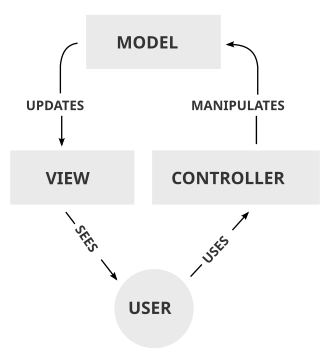
\includegraphics[width=0.9\textwidth]{architecture.png}
  \caption{System architecture diagram.}
  \label{fig:architecture}
\end{figure}

\section{Devices and Interfaces Used}
What devices did we use and for what purpose?
\begin{itemize}[itemsep=0.5em]
  \item \textbf{Mouse:} \ldots
  \item \textbf{Timer:} \ldots
  \item \textbf{Keyboard:} \ldots
  \item \textbf{RTC:} \ldots
\end{itemize}

\section{Differentiating Features}
What are the differentiating features of our project?

\section{Conclusion}
Summarize achievements, limitations, and possible future extensions.

\end{document}
